\chapter{Tracing Type Stability: An Empirical Study}\label{sec:empirical}

Anecdotal evidence suggests that type stability is discussed in the
Julia community, but does Julia code exhibit the properties of stability
and groundedness in practice? And if so, are there any indicators correlated with
instability and ungroundedness? To find out, we ran a dynamic analysis on a
corpus of Julia packages. All the packages come from the main language registry
and are readily available via Julia's package manager; registered packages have
to pass basic sanity checks and usually have a test suite.

The main questions of this empirical study are:
\begin{enumerate}
\item How uniformly are type stability and groundedness spread over Julia packages?
  How much of a difference can users expect from different packages?
\item Are package developers aware of type stability?
\item Are there any predictors of stability and groundedness in the code and do
  they influence how type-stable code looks?
\end{enumerate}

\section{Methodology}

We take as our main corpus the 1000 most starred (using GitHub stars) packages
from the Julia package registry; as of the beginning of 2021, the registry
contained about 5.5K packages. The main corpus is used for an automated,
high-level, aggregate analysis. We also take the 10 most starred packages from
the corpus to perform finer-grained analysis and manual inspection. Out of the
1000 packages in the corpus, tests suits of only \goodpkgsnum succeeded on
\juliaversion, so these \goodpkgsnum comprise our final corpus. The reasons of
failures are diverse, spanning from missing dependencies to the absence of
tests, to timeout.

For every package of interest, the dynamic analysis runs the package test suite,
analyzes compiled method instances, and records information relevant to
type stability and groundedness. Namely, once a test suite runs to completion,
we query Julia's virtual machine for the current set of available method
instances, which represent instances compiled during the tests' execution. To
avoid bias towards the standard library, we remove instances of methods defined in
standard modules, such as \c{Base}, \c{Core}, etc., \ADD{which typically leaves
us with several hundreds to several thousands of instances.}
For these remaining instances,
we analyze their type stability and groundedness. As type information is not
directly available for compiled, optimized code, we retrieve the original method
of an instance and run Julia's type inferencer to obtain each register's type,
similarly to the \jules model. In rare cases, type inference may fail;
on our corpus, this almost never happened, with at most 5 failures per package.
With the inference results at hand, we check the concreteness of the register
typing and record a yes/no answer for both stability and groundedness. In
addition to that, several metrics are recorded for each method:
method size, the number of gotos and returns in the body, whether the method has
varargs or \c{@nospecialize} arguments\footnote{\texttt{@nospecialize} tells the
compiler to \emph{not} specialize for that argument and leave it abstract.}, and
how polymorphic the method is, i.e. how many instances were compiled for it.
This information is then used to identify possible correlations between the
metrics and stability/groundedness.

To get a better understanding of type stability and performance, we employ
several additional tools to analyze the 10 packages. For example, we look at
their documentation, especially at the stated goals and domain of a package, and
check the Git history to see if and how type stability is mentioned in the
commits.

\begin{table}[t]\small
\caption{Aggregate statistics for stability and groundedness}%
\label{empirical:fig:all}
\begin{tabular}{@{}lrr@{}}
\toprule
          & \multicolumn{1}{c}{Stable} & \multicolumn{1}{c}{Grounded} \\ \midrule
Mean      & 74\%                       & 57\%                         \\
Median    & 80\%                       & 57\%                         \\
Std. Dev. & 22\%                       & 24\%                         \\ \bottomrule
\end{tabular}
\end{table}

\section{Package-Level Analysis}

The aggregate results of the dynamic analysis for the \goodpkgsnum packages are
shown in Table~\ref{empirical:fig:all}: 74\% of method instances in a package
are stable and 57\% grounded, on average; median values are close to the means.
The standard deviation is noticeable, so even on small samples of packages, we
expect to see packages with large deflections from the means.

A more detailed analysis of the 10 most starred packages, in alphabetical order,
is shown in Table~\ref{empirical:fig:top}. A majority of these packages have
stability numbers very close to the averages shown above, with the exception of
Knet, which has only 16\% of stable and 8\% of grounded instances.


\begin{table}[h]\small
\caption{Stability, groundedness, and polymorphism in 10 popular Juila packages}%
\label{empirical:fig:top}
\begin{tabular}{@{}lrrrrrr@{}}
\toprule
\multicolumn{1}{c}{Package} & \multicolumn{1}{c}{Methods} & \multicolumn{1}{c}{Instances} & \multicolumn{1}{c}{Varargs} & \multicolumn{1}{c}{Stable} & \multicolumn{1}{c}{Grounded} \\ \midrule
{\footnotesize DifferentialEquations}       & 1355                        & 7381                          & 3\%                         & 70\%                       & 44\%                         \\
Flux                        & 381                         & 4288                          & 13\%                        & 76\%                       & 70\%                         \\
Gadfly                      & 1100                        & 4717                          & 10\%                         & 81\%                       & 58\%                         \\
Gen                         & 973                         & 2605                          & 2\%                         & 64\%                       & 43\%                         \\
Genie                       & 532                         & 1401                          & 12\%                        & 93\%                       & 78\%                         \\
IJulia                      & 39                          & 136                           & 8\%                         & 84\%                       & 60\%                         \\
JuMP                        & 2377                        & 36406                         & 7\%                        & 83\%                       & 63\%                         \\
Knet                        & 594                         & 9013                          & 7\%                         & 16\%                       & 8\%                          \\
Plots                       & 1167                        & 5377                          & 8\%                         & 74\%                       & 58\%                         \\
Pluto                       & 727                         & 2337                          & 4\%                         & 80\%                       & 66\%                         \\ \bottomrule
\end{tabular}

\end{table}

The Knet package is a type stability outlier. A quick search over project's
documentation and history shows that the only kind of stability ever mentioned
is numerical stability; furthermore, the word ``performance'' is mostly used to
reference the performance of neural networks or CUDA-related utilities. Indeed,
the package primarily serves as a communication layer for a GPU; most
computations are done by calling the CUDA API for the purpose of building deep
neural networks. Thus, in this specific domain, type stability of Julia code
appears to be irrelevant.

On the other side of the stability spectrum is the 93\% stable (78\% grounded)
Genie package, which provides a web application framework. Inspecting the
package,
%
we can confirm that its developers were aware of type stability and
intentional about performance.
%
For example, Genie's Git history contains several commits mentioning (improved)
``type stability.''
The project README file states that the authors build upon
\begin{quote}
\itshape ``Julia's strengths (high-level, high-performance, dynamic, JIT compiled).''
\end{quote}
Furthermore, the tutorial claims:
\begin{quote}
\itshape ``Genie's goals: unparalleled developer productivity, excellent run-time
performance.''
\end{quote}

\paragraph{Type stability (non-)correlates}
One parameter that we conjectured may correlate with stability is the average
number of method instances per method (Inst/Meth column of
Table~\ref{empirical:fig:top}), as it expresses the amount of polymorphism
discovered in a package. Most of the packages compile just 2--4 instances per
method on average, but Flux, JuMP, and Knet have this metric 5--6 times higher,
with JuMP and Knet exploiting polymorphism the most, at 15.3 and 15.2
instances per method, respectively. The latter may be related to the very low type stability
index of Knet. However, the other two packages are more stable than the overall
average. Analyzing JuMP and Flux further, we order their methods by the number
of instances. In JuMP, the top 10\% of most instantiated methods are 5\% less
stable and grounded than the package average, whereas in Flux, the top 10\% have
about the same stability characteristics as on average. Overall, we cannot
conclude that method polymorphism is related to type stability.

Another dimension of polymorphism is the variable number of arguments in a
method (Varargs column of Table~\ref{empirical:fig:top}). We looked into three
packages with a higher than average (9\%) number of varargs methods in the 10
packages: Flux, Gadfly and Genie. Relative to the total number of methods, Flux has the most
varargs methods---13\%---and those methods are only 55\% stable and 44\%
grounded, which is a significant drop of 21\% and 26\% below this package's
averages. However, the other two packages have higher-than-package-average
stability rates, 82\% (Gadfly) and 99\% (Genie), with groundedness being high in
Genie, 93\%, and low in Gadfly, 38\%. Again, no general conclusion about the
relationship between varargs methods and their stability can be made.

\section{Method-Level Analysis}

\MODIFY{
In this section, we inspect stability of individual methods in its possible
relationship with other code properties like size, control flow (number of goto
and return statements), and polymorphism (number of compiled instances and varargs).
Our analysis consists of two steps: first, we plot histograms
showing the number of methods with particular values of properties, and second,
we manually sample some of the methods with more extreme characteristics.
}

\subsection{Graphical Analysis}
\label{sssect:graphs}

We use two-dimensional histograms like those presented in
Fig.~\ref{figs:size:Pluto:main} to discover possible relationships between stability
of code and its other properties. The vertical axis measures stability (on the
left diagram) or groundedness (on the right): $1$ means that all recorded
instances of a method are stable/grounded, and $0$ means that none of them are.
The horizontal axis measures the property of interest; in the case of
Fig.~\ref{figs:size:Pluto:main}, it is method size (actual numbers are not
important here: they are computed from Julia's internal representation of source
code). The color of an area reflects how many methods have characteristics
corresponding to that area's position on the diagram; e.g.\ in
Fig.~\ref{figs:size:Pluto:main}, the lonely yellow areas indicate that there are about
500 (400) small methods that are stable (grounded).

\begin{figure}[h]
     \begin{subfigure}[b]{0.48\textwidth}
       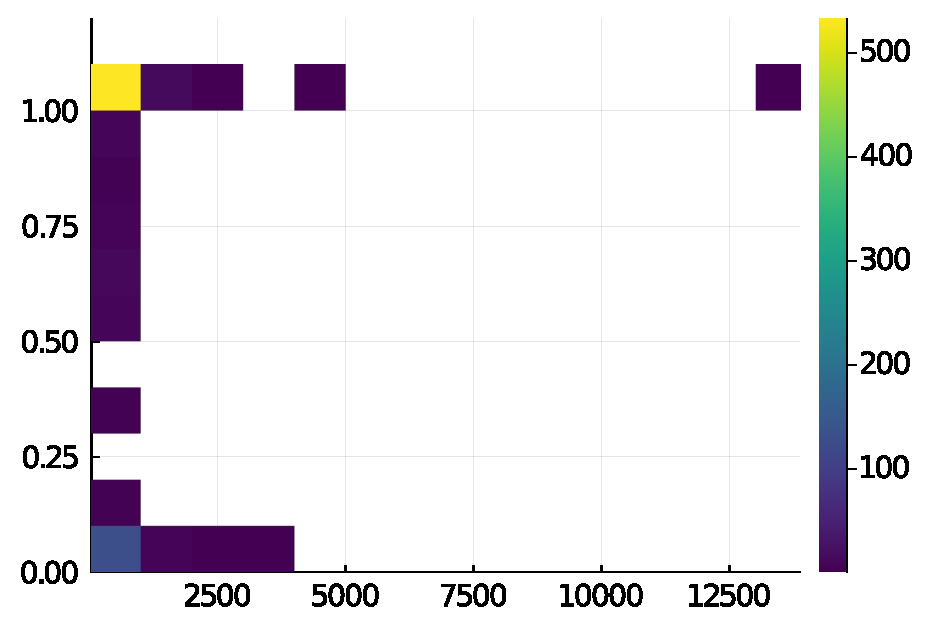
\includegraphics[width=\textwidth]{figs/Pluto-size-vs-stable.pdf}
     \end{subfigure}
     \ \ \
     \begin{subfigure}[b]{0.48\textwidth}
       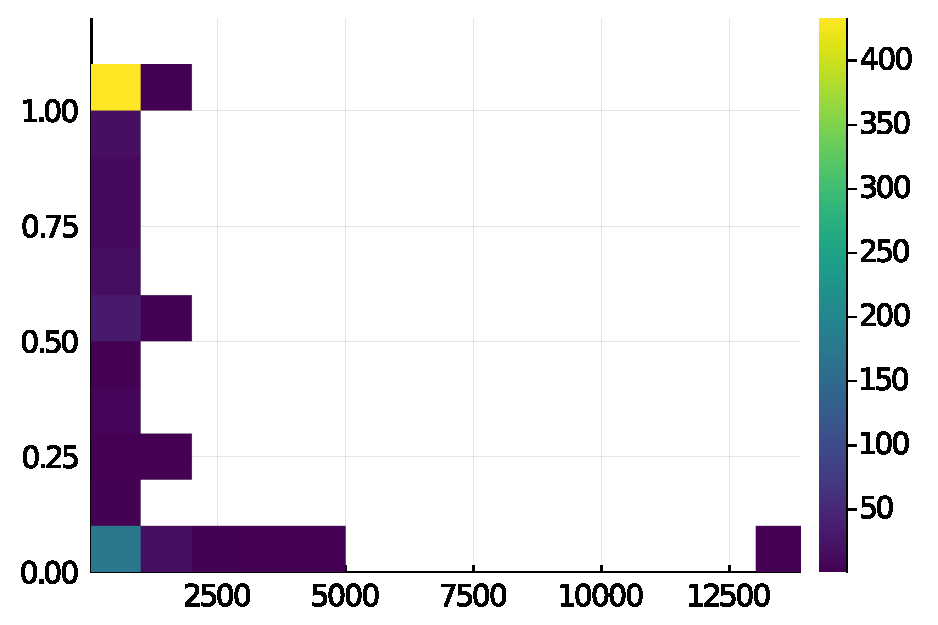
\includegraphics[width=\textwidth]{figs/Pluto-size-vs-grounded.pdf}
     \end{subfigure}
\caption{Stability (left, OY axis) and groundedness (right, OY) by method size (OX) in Pluto}%
\Description{Stability and groundedness by method size in Pluto}%
\label{figs:size:Pluto:main}
\end{figure}

We generate graphs for all of the 10 packages listed in
Table~\ref{empirical:fig:top}, for all combinations of the properties of
interest\PAPERVERSIONINLINE{; the graphs are available in the extended
version~\cite{oopsla21jules:arx}}{; the graphs are provided in \appref{sec:app}}.
Most of the graphs look very similar to the ones from
Fig.~\ref{figs:size:Pluto:main}, which depicts Pluto---a package for creating
Jupyter-\hspace{0pt}like notebooks in Julia. In the following paragraphs, we
discuss features of these graphs and highlight the discrepancies.

The first distinctive feature of the graphs is the hot area in the top-left
corner: most of the 10 packages employ many small, stable/grounded methods;
the bottom-left corner is usually the second-most hot, so a significant number
of small methods are unstable/ungrounded. For the Knet package,
these two corners are reversed; for DifferentialEquations, they are reversed
only on the groundedness plot. Both of these facts are not surprising after seeing
Table~\ref{empirical:fig:top}, but having a visual tool to discover such facts
may be useful for package developers.

The second distinctive feature of these graphs is the behavior of large,
ungrounded methods (bottom-right part of the right-hand-side graph). The
``tail'' of large methods on the groundedness graphs almost always lies below
the $1$-level; furthermore, larger methods tend to be less grounded.
However, if we switch from groundedness to stability plots, a large portion of
the tail jumps to the $1$-level. This means larger methods are unlikely to be
grounded (as expected, because of the growing number of registers), but they
still can be stable and thus efficiently used by other methods. Pluto provides a
good example of such a method: its \c{explore!} method of size 13003 (right-most
rectangle on Fig.~\ref{figs:size:Pluto:main}, 330 lines in the source code) analyzes
Julia syntax trees for scope information with a massive \c{if/else if/..} statement.
This method has a very low chance of being grounded, and it was not grounded on the
runs we analyzed. However, the method has a concrete return type annotation, so
Julia (and the programmer) can easily see that it is stable.

%% PLZ, DO NOT DELETE THIS
% Plots where the size axis is replaced with the number of branching or return
% instructions have a technical difference from what we see on
% Fig.~\ref{figs:size:Pluto:main} in that they reflect individual method instances
% instead of methods because due to Julia's simple optimizer, which kicks i
% when the main optimizer is turned off by our demand, instances of a method can
% have different number of those instructions. As a consequence, all squares on
% the histograms lie either on $1$-level or $0$-level. Otherwise, the picture is
% similar to Fig.~\ref{figs:size:Pluto:main} in the two distinctive feature discussed
% above.

In the case of the number of gotos and returns, the plots are largely similar
to the ones for method size, but they highlight one more package with low
groundedness. Namely, the Gen package (aimed at probabilistic
inference~\cite{JuliaGenPkgPub2019}) has the hottest area in the bottom-left
corner, contrary to the first general property we identified for the size-based
plots. Recall (Tables \ref{empirical:fig:all} and \ref{empirical:fig:top}) that
Gen's groundedness is 14\% less than the average on the whole corpus of
\goodpkgsnum packages.

\subsection{Manual Inspection}

\ADD{
To better understand the space of stable methods,
we performed a qualitative analysis of a sample of stable methods that
have either large sizes or many instances.

Many large methods have one common
feature: they often have a return type ascription on the method header of
the form:
}
\begin{lstlisting}[language=julia]
function f(...) :: Int
  ...
end
\end{lstlisting}
\ADD{
These ascriptions are a relatively new tool in Julia, and they are used only
occasionally, in our experience. An ascription makes the Julia compiler insert implicit
conversions on all return paths of the method. Conversions are user extendable:
if the user defines type \c{A}, they can also add methods of a special
function \c{convert} for conversion to \c{A}. This function will be called
when the compiler expects \c{A} but infers a different type, for example,
if the method returns \c{B}.
If the method returns \c{A}, however, then \c{convert} is a no-op.

Type ascriptions may be added simply as documentation, but they can also
be used to turn type instability into a run-time error:
if the ascribed type is concrete and a necessary conversion is not available,
the method will fail. This provides a useful, if
unexpected, way to assure that a large method never becomes unstable.

While about 85\% of type-stable methods in the top 10 packages are uninteresting
in that they always return the same type, sampling the rest illuminates
a clear pattern: the methods resemble what we
are used to see in statically typed languages with parametric polymorphism. Below
is a list of categories that we identify in this family.
}

\begin{itemize}

\lstset{basicstyle=\footnotesize\ttfamily,linewidth=.93\textwidth}

\ADD{
\item
  Various forms of the identity function---a surprisingly popular function that
  packages keep reinventing. In an impure language, such as Julia, an identity
  function can produce various side effects.
  For example, the Genie package adds a caching effect to
  its variant of the identity function:
}
\begin{lstlisting}[language=julia]
# Define the secret token used in the app for encryption and salting.
function secret_token!(value::AbstractString=Generator.secret_token())
  SECRET_TOKEN[] = value
  return value
end
\end{lstlisting}

\ADD{
\item
  Container manipulations for various kinds of containers, such as arrays, trees, or
  tuples. For instance, the latter is exemplified by the following function
  from Flux, which maps a tuple of functions by applying them to the given argument:
  %\clearpage
  % Oh, no! Manual page breaking makes me sad! -- Artem
}
\begin{lstlisting}[language=julia]
function extraChain(fs::Tuple, x)
  res = first(fs)(x)
  return (res, extraChain(Base.tail(fs), res)...)
end
extraChain(::Tuple{}, x) = ()
\end{lstlisting}

\ADD{
\item
  Smart constructors for user-defined polymorphic structures. For example, the following
  convenience function from JuMP creates an instance of the
  \c{VectorConstraint} structure with three fields, each of which is polymorphic:
}
\begin{lstlisting}[language=julia]
function build_constraint(_error::Function, Q::Symmetric{V,M}, ::PSDCone)
        where {V<:AbstractJuMPScalar,M<:AbstractMatrix{V}}
    n = LinearAlgebra.checksquare(Q)
    shape = SymmetricMatrixShape(n)
    return VectorConstraint(
        vectorize(Q, shape),
        MOI.PositiveSemidefiniteConeTriangle(n),
        shape)
end
\end{lstlisting}

\ADD{
\item
  Type computations---an unusually wide category for a dynamically typed
  language. Thus, for instance, the Gen package defines a type that represents generative
  functions in probabilistic programming, and a function that extracts the
  return and argument types:
}
\begin{lstlisting}[language=julia]
# Abstract type for a generative function with return value type T and trace type U.
abstract type GenerativeFunction{T,U <: Trace} end
get_return_type(::GenerativeFunction{T,U}) where {T,U} = T
get_trace_type(::GenerativeFunction{T,U}) where {T,U} = U
\end{lstlisting}

\lstset{linewidth=\textwidth}

\end{itemize}

\section{Takeaways}

Our analysis shows that a Julia user can expect mostly stable (74\%) and
somewhat grounded (57\%) code in widely used Julia packages. If the authors
are intentional about performance and stability, as demonstrated by the Genie
package, those numbers can be much higher. Although our sample of packages is
too small to draw strong conclusions, we suggest that several factors can be
used by a Julia programmer to pinpoint potential sources of instability in their
package. For example, in some cases, varargs methods might indicate instability.
Large methods, especially ones with heavy control flow,
tend to not be type grounded but often are stable; in particular,
if they always return the same concrete type.
Finally, although highly polymorphic methods are neither stable nor unstable
in general, code written in the style of parametric polymorphism
often suggests type stability.

Our dynamic analysis and visualization code is written in Julia (and some bash
code), and relies on the vanilla Julia implementation. Thus, it can be employed
by package developers to study type instability in their code, as well as check
for regressions.
